\documentclass[12pt]{article}
%\include{amsfonts}
\usepackage{amssymb,amsmath,amsthm,latexsym,epsfig,euscript,multicol}
\usepackage{enumitem}
\usepackage[utf8x]{inputenc}
\usepackage{booktabs}
\usepackage{babel}[spanish]
\usepackage{tikz}
% \usepackage{enumerate}

% Caracteres especiales
\def\A{\mathbb{A}}
\def\C{\mathbb{C}}
\def \N{\mathbb{N}}
\def \P{\mathbb{P}}
\def \Q{\mathbb{Q}}
\def \R{\mathbb{R}}
\def \Z{\mathbb{Z}}
\def \sen{\textrm{sen}}

\theoremstyle{definition}
\newtheorem{ejer}{Ejercicio}
\newcommand{\bej}{\begin{ejer}}
\newcommand{\fej}{\end{ejer}}

\def\dt{\Delta t}
\def\dx{\Delta x}
%\DeclareUnicodeCharacter{2212}{-}

\topmargin-2cm \vsize 29.5cm \hsize 21cm
\setlength{\textwidth}{16.75cm}\setlength{\textheight}{23.5cm}
\setlength{\oddsidemargin}{0.0cm}
\setlength{\evensidemargin}{0.0cm}


\begin{document}

%----------------------------------------------------------
%Encabezado:

\centerline{{\small Universidad de Buenos Aires - Facultad de Ciencias Exactas y Naturales - Depto. de Matemática}}

\vskip 0.2cm

\hrule

\vskip 0.2cm

 \centerline{{\bf\Large{\sc Investigación Operativa}}}

 \vskip 0.2cm

 \centerline{\ttfamily Segundo Cuatrimestre 2025}

\vskip 0.2cm

 \hrule

 \bigskip
 \centerline{\bf Práctica 4: Grafos}
 \bigskip

%--------------------------------------------------------- 
% 1
\bej
Sea $G$ un grafo que no tiene vértices aislados y tiene $m$ aristas. Determine el mayor número de vértices que puede tener $G$. Si $m = 50$, ¿cuál es el máximo número de vértices teniendo todos grado al menos $3$?
\fej
%--------------------------------------------------------- 

\bej
Sea $G = (V, E)$ un digrafo (grafo dirigido). Se definen para $v \in V$ , $d_s(v)$ y $d_e(v)$ como el número de aristas que salen (respectivamente llegan) de $v$. Pruebe que:
\[ \sum_{v\in V} d_s(v) = \sum_{v\in V} d_e(v)\]
\fej

%--------------------------------------------------------- 
\bej
Un grafo $G$ se dice autocomplementario si es isomorfo a su complemento $G$. Encuentre todos los grafos autocomplementarios con a lo sumo 5 vértices. Muestre que si un grafo autocomplementario tiene $n$ vértices, entonces es $n \equiv 0 \;(4)$ o $ n \equiv 1 \;(4)$.
\fej
%--------------------------------------------------------- 

\bej
Sean $G$ un grafo y $A$ su matriz de adyacencia. Pruebe que $A^n_{
i,j}$ coincide con la cantidad de
caminos (no necesariamente simples) de largo $n$ que unen el vértice $i$ con el vértice $j$.
\fej

%--------------------------------------------------------- 

\bej
\hspace{1em}

\begin{enumerate}
    \item Caracterice la matriz de adyacencia de un grafo bipartito.
    \item Pruebe que un grafo es bipartito si y sólo si para todo $n$ impar los elementos de la diagonal de $A^n$ son nulos, donde $A$ es la matriz de adyacencia del grafo.
\end{enumerate}
\fej
%--------------------------------------------------------- 

\bej
Pruebe que un grafo $G = (V, E)$ es conexo si y sólo si para toda partición de $V$ en dos subconjuntos $V_1$ y $V_2$ hay una arista de $G$ que une un vértice de $V_1$ con uno de $V_2$.
\fej

%--------------------------------------------------------- 
\bej
Pruebe que un grafo de $n$ vértices con grado al menos $\frac{n-1}{2}$ es conexo
\fej

%--------------------------------------------------------- 

\bej
Pruebe que un grafo de $n$ vértices que tiene más de $\frac{(n-1)(n-2)}{2}$ aristas es conexo.

\fej
%--------------------------------------------------------- 

\bej
Sea $G$ un grafo pesado y supongamos que los pesos son todos distintos. Pruebe que $G$ tiene un
único árbol generador mínimo.
\fej

%--------------------------------------------------------- 

\bej

Pruebe que en todo grafo conexo con más de un vértice hay al menos dos vértices que no son de corte (es decir, que al removerlos el grafo sigue siendo conexo).

\fej
%--------------------------------------------------------- 


\bej
Supongamos que se tienen cuatro aulas y las siguientes materias con sus respectivos horarios
para un mismo día:
\begin{table}[htpb!]
    \centering
    \begin{tabular}{lrlr}
        Análisis I & 8 a 13 hs. & Análisis II &  10 a 15 hs. \\
        Cálculo Avanzado & 14 a 19 hs. & Análisis Complejo & 11 a 16 hs. \\
        Probabilidad & 14 a 17 hs. & Investigación Operativa & 17 a 22 hs. \\
        Gometría Proyectiva & 14 a 19 hs. & Análisis Numérico & 14 a 19 hs. \\
    \end{tabular}
\end{table}
Modele como un problema de grafos y decida si existe una forma de asignar aulas de forma que se puedan dictar todas las materias respetando los horarios. 
\fej
%--------------------------------------------------------- 

\bej
Considere el siguiente grafo, conocido como $W_5$. Calcule el polinomio, número e índice cromático de G.

\begin{center}
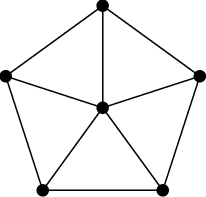
\includegraphics[scale=0.65]{Imagenes/w5.png}
\end{center}
\fej

%--------------------------------------------------------- 

\bej
Sea G el grafo que figura a continuación. Brinde dos cotas $\alpha$ y $\beta$, con $\beta < 5$, tales que $\alpha \leq \chi(G) \leq \beta $. Exhiba un coloreo utilizando $\alpha$ colores. Corrobórelo mediante el algoritmo de conexión - contracción.
\begin{center}
    
\includegraphics[scale=0.3]{Imagenes/grafo_1.png}
\end{center}
\fej

%--------------------------------------------------------- 

\bej
Determine el polinomio cromático del siguiente grafo de manera directa y verifíquelo mediante el algoritmo de conexión - contracción.

\begin{center}
    
\includegraphics[scale=0.3]{Imagenes/grafo_2.png}
\end{center}
\fej

%--------------------------------------------------------- 

\bej
En una ciudad hay $N$ esquinas y $M$ calles. Conociendo el mapa de la ciudad, se busca decidir si
es posible colocar policías en algunas de las esquinas de manera que cada calle sea custodiada
por exactamente un policía (un policía custodia las calles que desembocan en la esquina en que
se encuentra). Modele el problema usando grafos.

\fej
%--------------------------------------------------------- 

\bej
Considere los siguientes dibujos:
\begin{center}
    
\includegraphics[scale=0.3]{Imagenes/grafo_3.png}
\end{center}

Empezando y terminando en el mismo vértice, ¿es posible reproducirlos sin levantar el lápiz?
Exprese el problema en términos de teoría de grafos.
\fej

%--------------------------------------------------------- 

\bej

Labyrinthroid es un videojuego en el cual, en cada nivel, se debe llegar a la meta atravesando un laberinto y derrotando enemigos inmóviles. Tanto el mapa del nivel como la posición de los enemigos son conocidos.
Se puede considerar como ejemplo el siguiente nivel:

\begin{center}
    \begin{tikzpicture}
        \fill[black!40!white] (3,2) rectangle (4,3);
        \fill[black!40!white] (3,0) rectangle (4,1);
        \fill[black!40!white] (1,0) rectangle (2,2);
        \draw[step=1cm,black,very thin] (0,0) grid (4,3);
        \node[inner sep=0pt] (protag) at (0.5, 0.5) {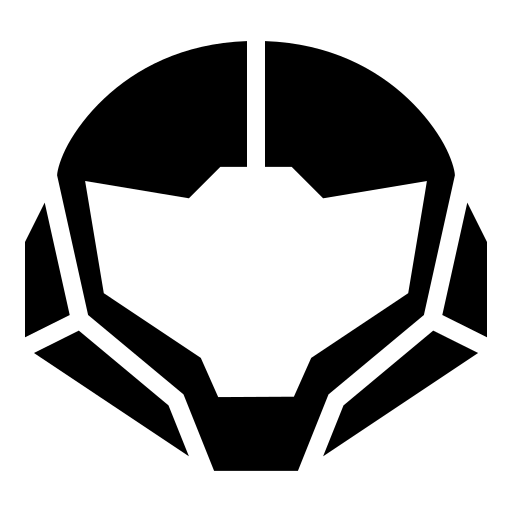
\includegraphics[scale=0.05]{Imagenes/protag.png}};
        \node[inner sep=0pt] (monster) at (2.5, 2.5) {
\includegraphics[scale=0.022]{Imagenes/monster.png}};
        \node[inner sep=0pt] (door) at (3.5, 1.5) {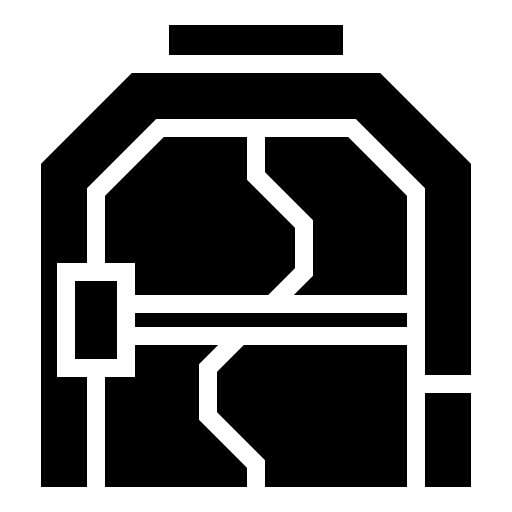
\includegraphics[scale=0.05]{Imagenes/airtight-hatch (1).png}};
        \node[inner sep=0pt] (arrow2) at (4.5, 1.5) {
\includegraphics[scale=0.025]{Imagenes/arrow.png}};
        \node[inner sep=0pt] (arrow) at (-0.5, 0.5) {
\includegraphics[scale=0.025]{Imagenes/arrow.png}};
    \end{tikzpicture}
\end{center}

Las reglas son las siguientes:
\begin{itemize}
    \item La protagonista puede moverse a un casillero adyacente en las direcciones $\uparrow, \rightarrow, \downarrow$
    o  $\leftarrow $, siempre y cuando no haya un obstáculo (casillero gris). Cada movimiento consume $1$
    unidad de tiempo.
    \item Moverse a/desde un casillero donde se encuentra un enemigo consume $2$ unidades de tiempo.
    \item
    La protagonista tiene la habilidad especial de transformar un obstáculo en un casillero común, pero puede utilizar
    esta habilidad a lo sumo una vez por nivel. Usar la habilidad no consume tiempo, pero desplazarse a/desde el nuevo
    casillero habilitado sí.
\end{itemize}
Uno de los logros de Labyrinthroid es finalizar el juego en el menor tiempo posible. Dado un nivel, modelar el problema
de llegar a la meta en el menor tiempo posible como un problema en un grafo y proponer un algoritmo que utilice dicho
grafo para resolverlo en tiempo polinomial.

\fej

%---------------------------------------------------------

\bej

Una empresa tecnológica opera una red distribuida de servidores que se comunican entre sí. Cada enlace entre dos
servidores tiene un tiempo de transmisión.


\begin{enumerate}
    \item En momentos de congestión, el sistema debe elegir el camino de menor tiempo de transmisión para enviar un paquete desde
un servidor origen hacia un servidor destino. Modelar el problema como un problema de grafos. ¿Qué algoritmo
    utilizarías para encontrar el camino con menor tiempo de transmisión desde un servidor $s$ al resto de los
    servidores?
    \item Supongamos que en vez del tiempo de transmisión entre los servidores, tenemos la probabilidad de
    entrega exitosa de paquetes. La probabilidad entre los enlaces es independiente: si $p_{uv}$ es la probabilidad
    de una entrega exitosa del servidor $u$ al servidor $v$ y $p_{vw}$ la probabilidad de entrega exitosa desde $v$ a
    $w$, entonces enviar un paquete por el camino $u\rightarrow v\rightarrow w$ tiene probabilidad de éxito
    $p_{uv}\cdot p_{vw}$.
    Dado un servidor $s$, proporner una manera de hallar el camino con la probabilidad de éxito máxima al resto de
    los servidores.
\end{enumerate}

\fej

%---------------------------------------------------------
%\bej
%La red de transportes de una provincia deja mucho que desear. Concretamente, la provincia
%tiene $N$ ciudades conectadas por $M$ líneas de colectivos. El colectivo de la $i$-ésima línea tiene
%una capacidad determinada $C_i$ de pasajeros. Un tour por la provincia es una secuencia válida de
%viajes en colectivo que empieza en la ciudad $1$ y termina en la ciudad $N$. Si queremos llevar a
%un grupo de $P$ personas a conocer todas las ciudades de la provincia, ¿cuál es el mínimo número
%de tours que hay que realizar?
%\fej
%
%%---------------------------------------------------------
%
%\bej
%Considere la siguiente tabla con el tipo de cambio de algunas monedas (al 15/10/19):
%
%\begin{table}[htpb!]
%    \centering
%    \begin{tabular}{|c|c|c|c|c|}\hline
%        Tasa de cambio & Peso argentino  &  Dólar  & Peso chileno & Real \\\hline
%         Peso argentino & $1$ & $0.0179$ & $12.27$  & $0.0746$ \\\hline
%         Dólar &  $59.50$ & $1$ & $715.90$  & $4.15$ \\\hline
%         Peso Chileno & $0.082$  & $0.014$ & $1$ &  $0.0058$\\\hline
%         Real & $15.40$  & $0.24$  & $172.34$ & $1$ \\\hline
%    \end{tabular}
%\end{table}
%
%Modele el problema de cambiar de forma óptima 1000 pesos argentinos a dólares en términos de
%grafos. ¿Es posible hacer una sucesión de cambios en las que se termine con más de 1000 pesos
%argentinos?
%\fej
%
%%---------------------------------------------------------
%
%\bej
%Se cuenta con $N$ cubos de madera de distintos tamaños. Cada cara de los cubos está coloreada.
%Modele el problema de construir la torre de cubos más alta posible si no se puede apilar un cubo
%sobre otro más chico y además los colores de dos caras superpuestas tienen que coincidir
%\fej

\end{document}
%--------------------------------------------------------- 